\documentclass [10pt,a4paper,tikz] {book}
\usepackage{tikz}
\usepackage{booktabs}
\usepackage{siunitx}
\usepackage{amsmath}
\usepackage{relsize}
\usepackage{caption}
\usepackage{mwe}
\usepackage{booktabs}
\usepackage{amssymb}
\usepackage{wrapfig}
\usepackage{lipsum}
\usetikzlibrary{arrows,automata}





\let\oldemptyset\emptyset
\let\emptyset\varnothing

\begin{document}

\title{Project of \LaTeX \\ Page 97 to 100
}

\author{Mohammadamin Raisi\\ Student Number :970087192 \\ Unit : Tehran Shomal - Shahriar
}

\maketitle



\renewcommand{\thepage}{Page \arabic{page} $|$ Introduction to Automata Theory, Formal Languages and Computation }

\textbf{Solution :}

\begin{center}

\begin{tabular}{ccc}

\toprule
\multicolumn{3}{c}{Next State} \\

\cmidrule(r){2-3}
 Present State  & 0  & 1 \\
    \midrule
    $[{q}_{0}]$ & $[{q}_{0}$,${q}_{3}]$ & $[{q}_{0}$,${q}_{1 }]$\\
    $[{q}_{0}$,${q}_{3}]$ & $[{q}_{0}$,${q}_{3}$,${q}_{4}]$ & $[{q}_{0}$,${q}_{1}]$ \\
    $[{q}_{0}$,${q}_{3}$,${q}_{4}]$ & $[{q}_{0}$,${q}_{3}$,${q}_{4}]$ & $[{q}_{0}$,${q}_{1}$,${q}_{4}]$ \\
    $[{q}_{0}$,${q}_{1}$,${q}_{4}]$ & $[{q}_{0}$,${q}_{3}$,${q}_{4}]$ & $[{q}_{0}$,${q}_{1}$,${q}_{4}]$ \\
    $[{q}_{0}$,${q}_{1}]$ & $[{q}_{0}$,${q}_{3}]$ & $[{q}_{0}$,${q}_{1}]$ \\
    \bottomrule


\end{tabular}

\end{center}



For simplification, let us replace $[{q}_{0}]$ by A, $[{q}_{0},{q}_{3},]$ by B, $[{q}_{0}$,${q}_{3}$,${q}_{4}]$ by C, $[{q}_{0}$,${q}_{1}$,${q}_{4}]$ by D, and
$[{q}_{0}$,${q}_{1}]$ by E. Here, A is the initial state, and C and D are the final states as they contain the state ${q}_{0}$.
The simplified DFA is

\begin{center}

\begin{tabular}{llr}
\toprule
\multicolumn{2}{r}{Next State} \\
\cmidrule(r){2-3}
 Present State & 0 {\hspace{10\tabcolsep}} & 1 \\
    \midrule
    A & B & E \\
    B & C & E \\
    C & C & D \\
    D & C & D \\
    E & B & E \\

    \bottomrule


\end{tabular}

\end{center}

6. Convert the following NFA to an equivalent DFA.


\textbf{Solution :}

\begin{center}

\begin{tabular}{ccc}
\toprule
\multicolumn{3}{l}{$\sum$} \\
\cmidrule(r){1-1}
 States & 0 & 1 \\
    \midrule
    ${q}_{0}$ & ${q}_{0}$ & ${q}_{0}$,${q}_{1}$ \\
    ${q}_{1}$ & ${q}_{2}$ & ${q}_{2}$ \\
    ${q}_{0}$ & - & ${q}_{1}$ \\

    \bottomrule


\end{tabular}

\end{center}

($[{q}_{0}]$ is the initial state and $[{q}_{1}]$ is the final state)\\
\textbf{Solution:} Conversion is done in the following ways:
\\

\begin{center}

\begin{tabular}{ccc}
\toprule
\multicolumn{3}{l}{$\sum$} \\
\cmidrule(r){1-1}
 States & 0 & 1 \\
    \midrule
    $[{q}_{0}]$ & $[{q}_{0}]$ & $[{q}_{0}$,${q}_{1}]$ \\
    $[{q}_{0}$,${q}_{1}]$ & $[{q}_{0}$,${q}_{2}]$ & $[{q}_{0}$,${q}_{1}$,${q}_{2}]$ \\
    $[{q}_{0}$,${q}_{1}$,${q}_{2}]$ & $[{q}_{0}$,${q}_{2}]$ & $[{q}_{0}$,${q}_{1}$,${q}_{2}]$ \\
    $[{q}_{0}$,${q}_{2}]$ & $[{q}_{0}]$ & $[{q}_{0}$,${q}_{1}$,${q}_{2}]$ \\

    \bottomrule


\end{tabular}

\end{center}

Rename $[{q}_{0}]$ as A, $[{q}_{0}$,${q}_{1 }]$ as B, $[{q}_{0}$,${q}_{1}$,${q}_{2}]$ as C, and $[{q}_{0}$,${q}_{2}]$ as D. The beginning state is A, and
final states are B and C.

\begin{center}

\begin{tabular}{ccc}
\toprule
\multicolumn{3}{l}{$\sum$} \\
\cmidrule(r){1-1}
 States & 0 & 1 \\
    \midrule
    A & A & B \\
    B & D & C \\
    C & D & C \\
    D & A & C \\

    \bottomrule


\end{tabular}

\end{center}

7. Convert the following NFA to an equivalent DFA.
[UPTU 2005]

\begin{center}

\begin{tabular}{ccc}


\toprule
\multicolumn{3}{l}{$\sum$} \\
\cmidrule(r){1-1}
 States & 0 & 1 \\
    \midrule
    p & \{q,s\} & \{q\} \\
    q & \{e\} & \{q,r\} \\
    r & \{s\} & \{p\} \\
    s & $\emptyset$ & \{p\} \\

    \bottomrule


\end{tabular}

\end{center}



where p is the initial state and q and s are the final states.
\textbf{Solution:
}
\begin{center}

\begin{tabular}{ccc}


\toprule
\multicolumn{3}{l}{$\sum$} \\
\cmidrule(r){1-1}
 States & 0 & 1 \\
    \midrule
    \{p\} & \{q,s\} & \{q\} \\
    \{q\} & \{r\} & \{q,r\} \\
    \{r\} & \{s\} & \{p\} \\
    \{s\} & $\emptyset$ & \{p\} \\
    \{q,r\} & \{r,s\} & \{p,q,r\} \\
    \{r,s\} & \{s\} & \{p\} \\
    \{p,q,r\} & \{q,r,s\} & \{p,q,r\} \\
    \{q,r,s\} & \{r,s\} & \{p,q,r\} \\
    \{q,s\} & \{r\} & \{p,q,r\} \\
    \{$\emptyset$\}& \{$\emptyset$\} & \{$\emptyset$\} \\

    \bottomrule


\end{tabular}

\end{center}
Here \{p\}\} is the beginning state and \{q\}, \{s\}, \{q, r\}, \{r, s\}, \{p, q, r\}, \{q, r, s\}, and \{q, s\} are
the final states. $\oldemptyset$ is the dead state.\\
8. Construct a DFA equivalent to the following NDFA given in the following figure.
[UPTU 2004]



\begin{center}

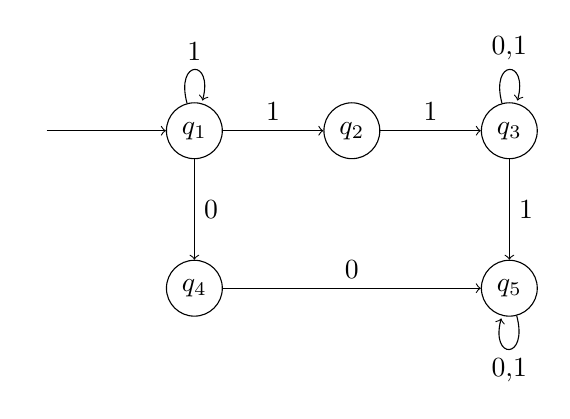
\begin{tikzpicture}[->,main/.style = {draw,circle},node distance = 2cm , auto]

\node[main] (1) {$q_1$};
\node[main] (2) [right of=1] {$q_2$};
\node[main] (3) [right of=2] {$q_3$};
\node[main] (4) [below of=1] {$q_4$};
\node[main] (5) [below of=3] {$q_5$};
\node (6) [left of=1] {};


\path (1) edge node {1} (2);
\path (2) edge node {1} (3);
\path (3) edge node {1} (5);
\path (4) edge node {0} (5);
\path (6) edge node {} (1);
\path (1) edge node {0} (4);



\path (1) edge [loop above] node {1} (1);
\path (3) edge [loop above] node {0,1}(3);
\path (5) edge [loop below] node {0,1}(5);


\end{tikzpicture}

\end{center}

\textbf{Solution:} The tabular representation of the NDFA is

\begin{center}

\begin{tabular}{ccc}
\toprule
\multicolumn{2}{r}{Next State} \\
\cmidrule(r){2-3}
 Present State & 0 & 1 \\
    \midrule
    ${q}_{0}$ & ${q}_{3}$ & $\{{q}_{0}$,${q}_{1}\}$ \\
    ${q}_{1}$ & $\emptyset$ & ${q}_{2}$\\
    ${q}_{2}$& ${q}_{2}$ & $\{{q}_{2}$,${q}_{4}\}$ \\
    ${q}_{3}$ & ${q}_{4}$ & $\emptyset$ \\
    ${q}_{4}$& ${q}_{4}$ & ${q}_{4}$\\

    \bottomrule


\end{tabular}

\end{center}
(${q}_{0}$ is the initial state and ${q}_{4}$ is the final state)\\
The corresponding DFA is

\begin{center}

\begin{tabular}{ccc}


\toprule
\multicolumn{3}{l}{$\sum$} \\
\cmidrule(r){1-1}
 States & 0 & 1 \\
    \midrule
    $\{{q}_{0}\}$ & $\{{q}_{3}\}$ & $\{{q}_{0}$,${q}_{1}\}$ \\
    $\{{q}_{3}\}$ & $\{{q}_{4}\}$ & $\{\emptyset\}$\\
    $\{{q}_{4}\}$& $\{{q}_{4}\}$ & $\{{q}_{4}\}$ \\
    $\{{q}_{0}$,${q}_{1}\}$ & $\{{q}_{2}\}$ & $\{{q}_{2}$,${q}_{4}\}$ \\
    $\{{q}_{2}\}$ & $\{{q}_{2}\}$ & $\{{q}_{2}$,${q}_{4}\}$ \\
    $\{{q}_{2}$,${q}_{4}\}$ & $\{{q}_{2}$,${q}_{4}\}$ & $\{{q}_{2}$,${q}_{4}\}$ \\
    $\{\emptyset\}$ & $\{\emptyset\}$ & $\{\emptyset\}$\\
    \bottomrule


\end{tabular}

\end{center}

Here $\{{q}_{0}\}$ is the beginning state, and $\{{q}_{4}\}$, and $\{{q}_{0}$,${q}_{1}\}$ are the final states.\\
(Draw a transitional diagram to complete the answer.)\\
9. Find the minimal DFAs for the language L = $\{a^{n}b^{m},n\geq2,m\geq1\}$
\textbf{Solution}: All ‘a’ will appear before ‘b’. There is atleast 2 ‘a’ and 1 ‘b’. The DFA is the
following.


\begin{center}

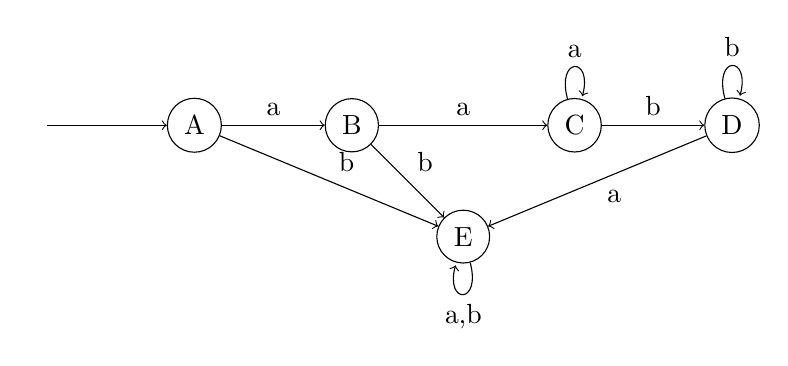
\begin{tikzpicture}[->,main/.style = {draw,circle},node distance = 2cm , auto]

\node[main] (e) {E};
\node[main] (b) [above left of=e] {B};
\node[main] (c) [above right of=e] {C};
\node[main] (a) [left of=b] {A};
\node[main] (d) [right of=c] {D};
\node (6) [left of=a] {};


\path (a) edge node {a} (b);
\path (a) edge node {b} (e);
\path (6) edge node {} (a);
\path (b) edge node {a} (c);
\path (b) edge node {b} (e);
\path (c) edge node {b} (d);
\path (d) edge node {a} (e);



\path (c) edge [loop above] node {a} (c);
\path (d) edge [loop above] node {b}(d);
\path (e) edge [loop below] node {a,b}(e);


\end{tikzpicture}

\end{center}

{10. Design a DFA for the language L = $\{0^{m}1^{n},m\geq0,n\geq1\}$ [JNTU 2007]\\


\begin{wrapfigure}{r}{3cm}
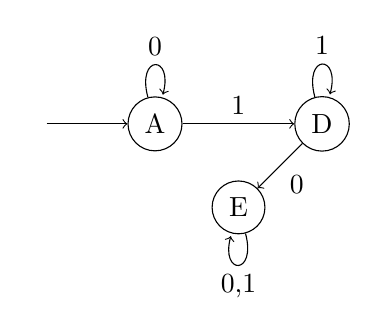
\begin{tikzpicture}[->,main/.style = {draw,circle},node distance = 1.5cm , auto]

\node[main] (e) {E};
\node[main] (a) [above left of=e] {A};
\node[main] (d) [above right of=e] {D};
\node (6) [left of=a] {};



\path (a) edge node {1} (d);
\path (d) edge node {0} (e);
\path (6) edge node {} (a);


\path (a) edge [loop above] node {0} (a);
\path (d) edge [loop above] node {1}(d);
\path (e) edge [loop below] node {0,1}(e);


\end{tikzpicture}

\begin{center}
 \textbf{Fig. 3.58 }
\end{center}

\end{wrapfigure}


\textbf{Solution}: All ‘0’s will appear before ‘1’. There is at least one
‘1’, but the number of ‘0’s may be zero. The DFA is shown in
Fig. 3.58.\\

11. Construct a DFA which accepts the set of all binary strings that,
interpreted as the binary representation of an unsigned decimal
integer, is divisible by 5.

[WBUT 2008]\\

\textbf{Solution:} For Mod 5, the remainders are 0, 1, 2, 3, and 4. We can assign the states as $q_0$, $q_1$, $q_2$,
$q_3$, and $q_4$.
\\For any binary string, if we add a bit at LSB, then the previous value becomes doubled. (Let
the string be 101. The decimal value is 5. If we add another 1 at LSB, the string becomes 1011.
The decimal value of the previous 101 becomes 10.)
\\In general, we can write that ‘n’ becomes 2n + b, where n is the previous number and b is the
added bit.

\begin{center}

(2n + b) mod 5 = 2n mod 5 + b mod 5

\end{center}
As b is either 0 or 1, b mod 5 = b.
2n mod 5 is any one of 0, 1, 2, 3, or 4, i.e., 2 X (state number) + a.
For this machine, the input alphabets are 0 and 1.

\begin{center}
$\delta$($q_0$, 0) $\rightarrow$ 2 × 0 + 0 = 0 means $q_0$\\
$\delta$($q_0$, 1) $\rightarrow$ 2 × 0 + 1 = 1 means $q_1$\\
$\delta$($q_1$, 0) $\rightarrow$ 2 × 1 + 0 = 2 means $q_2$\\
$\delta$($q_1$, 1) $\rightarrow$ 2 × 1 + 1 = 3 means $q_3$\\
$\delta$($q_2$, 0) $\rightarrow$ 2 × 2 + 0 = 4 means $q_4$\\
$\delta$($q_2$, 1) $\rightarrow$ 2 × 2 + 1 = 5\%5 = 0 means $q_0$\\
$\delta$($q_3$, 0) $\rightarrow$ 2 × 3 + 0 = 6\%5 = 1 means $q_1$\\
$\delta$($q_3$, 1) $\rightarrow$ 2 × 3 + 1 = 7\%5 = 2 means $q_2$\\
$\delta$($q_4$, 0) $\rightarrow$ 2 × 4 + 0 = 8\%5 = 3 means $q_3$\\
$\delta$($q_4$, 1) $\rightarrow$ 2 × 4 + 1 = 9\%5 = 4 means $q_4$\\
\end{center}




\end{document}​ 